\documentclass[10pt]{beamer}

\usepackage[utf8]{inputenc}
\usepackage{pgfpages}
\usepackage{dirtree}
\setbeamertemplate{note page}[plain]
\AtEndNote{\vfill \begin{center} mm:hh \end{center}}
\newcommand{\notedir}[1] {
  \note{\dirtree{#1}}}
\def \ion {$^{\circ}$ }
\usepackage{tcolorbox}
\usepackage{tikz}
\usepackage{tikz-3dplot}
\usetikzlibrary{intersections,calc,,angles,quotes,through}
\usepackage{amsmath}
\usepackage{graphicx}
\usepackage{cases}
\def \heart {\textcolor{blue}{$\heartsuit$} }
\def \C {\mathcal{C}}
\def \orthog {\underline{\perp}}
\def \arcos{\operatorname{arcos}}
\def \deg {^{\circ}}

\tcbset{%
	basic/.style={colframe=black,
		      colback=white,
		      top= 0mm,
		      bottom = 2mm,
		      boxsep=0mm
		      }
}
\tikzset{
    invisible/.style={opacity=0},
    visible on/.style={alt={#1{}{invisible}}},
    alt/.code args={<#1>#2#3}{%
      \alt<#1>{\pgfkeysalso{#2}}{\pgfkeysalso{#3}} % \pgfkeysalso doesn't change the path
    },
  }

    
\begin{document}  
    \beamertemplatenavigationsymbolsempty
    \setlength{\abovedisplayskip}{0pt}
    \setlength{\belowdisplayskip}{0pt}
    \frame{
	  
	  \frametitle{Q1 Juillet 2003.}
	  \renewcommand{\theenumi}{\alph{enumi})}
	  On considère un triangle $ABC$ dont les angles sont inférieurs à $120^{\circ}$. On construit
	  les triangles équilatéraux $ABC'$, $BCA'$ et $ACB'$ extérieurs à $ABC$. On note $I$
	  l’intersection de $AA'$ et $CC'$.
	  \begin{enumerate}
	   \item Démontrer que $|AA'|=|BB'| = |CC'|$.
	   \item Démontrer que $\widehat{BIC}=\widehat{BIA}=120^{\circ}$.
	   \item Démontrer que les droites $AA'$, $BB'$ et $CC'$ sont concourantes.
	  \end{enumerate}

	  \vfill
	  
	  \pause
	  % hypothèses et thèse
	  \begin{tcolorbox}[basic] 
	      \begin{columns}[t]
		 
		 \column{.5\textwidth}\centering
		      
		      \underline{Hypothèses} 
		      \begin{itemize}
		      \item $\Delta A'BC,\Delta AB'C,\Delta ABC'$ équilatéraux.
		      \end{itemize}

		  
		  \column{.5\textwidth}\centering
		      
		      \underline{Thèse} \\
		      \smallskip
		      \begin{enumerate}
		       \item $|AA'|=|BB'| = |CC'|$,
		       \item $\widehat{BIC}=\widehat{BIA}=120^{\circ}$,
		       \item $AA',BB',CC'$ concourantes.
		      \end{enumerate}

		
	      \end{columns}
	  \end{tcolorbox}
	  \notedir{%
	.1 Énoncé.
	.2 Hypothèses (non visibles sur le dessin)..
	.2 Thèse..
	.2 Grand dessin.. 
	}
    }

    \frame{ 
	  % résolution ex1
	  \begin{columns}[t]
		\column{.537\textwidth}\centering 
		

			\underline{Dessin}\\
				  \vspace{-2mm}
				  \begin{figure}[h]
				  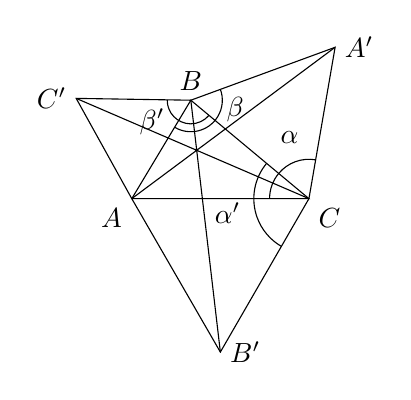
\begin{tikzpicture}[scale=0.5]
			          %projection ($(X)!(B')!(B)$)
			          %nommer chemin 'name path
			          %intersection \path [name intersections={of=d and gb,by=G}];
			          %animation  \draw[visible on=<1>] 
				  %           \draw[visible on=<{2,4}>]
				  %angle arc[radius = 6mm, start angle= 180, end angle= 225] node [below left,pos=0.3]{$\alpha$}
				  %angle \pic [draw, visible on=<2>, above left,"$\beta$", angle eccentricity=1.5] {angle = A'--A--B};
				  %TRIANGLE ABC
				  \coordinate[label=below left:$A$] (A) at (-1.5,0);
				  \coordinate[label=below right:$C$] (C) at (3,0);
				  \coordinate[label=above:$B$] (B) at (0,2.5);
				  \draw (A) -- (B) -- (C) -- cycle;
				  %ABC'
				  \draw (A) let \p1 = ($(B)-(A)$) in -- ++(119:{veclen(\x1,\y1)}) coordinate[label=left:$C'$](C') -- (B);
				  %A'BC
				  \draw (C) let \p1 = ($(B)-(C)$) in -- ++(80.19:{veclen(\x1,\y1)}) coordinate[label=right:$A'$] (A') -- (B);
				  %AB'C
				  \draw (A) let \p1 = ($(A)-(C)$) in -- ++(-60:{veclen(\x1,\y1)}) coordinate[label=right:$B'$] (B') -- (C);
				  %AA', BB', CC'
				  \draw (A) -- (A') (B) -- (B') (C) -- (C');
				  
				  %ANGLES
				  \pic [draw,visible on=<1>,"$\alpha$",above right, angle eccentricity=1.5] {angle = A'--C--A};
				  \pic [draw,visible on=<1>,"$\alpha '$", angle eccentricity=1.5,angle radius = 7mm] {angle = B--C--B'};
				  \pic [draw,visible on=<2>,"$\beta $",above right,angle eccentricity=1.3,angle radius = 4mm] {angle = A--B--A'};
				  \pic [draw,visible on=<2>,"$\beta '$",above left,angle eccentricity=2,angle radius = 3mm] {angle = C'--B--C};
				  \end{tikzpicture}
				  \end{figure}
				  \vspace{-3mm}
				  \begin{tcolorbox}[basic] 
				      
				    \smallskip
				    \underline{Hypothèses} 
				    \begin{enumerate}
				    \item $\Delta A'BC,\Delta AB'C,\Delta ABC'$ équilatéraux.
				    \end{enumerate}
							      
				    \underline{Thèse}
				    \renewcommand{\theenumi}{\alph{enumi})}
				    \begin{enumerate}
				    \item $|AA'|=|BB'| = |CC'|$,
				    \item $\widehat{BIC}=\widehat{BIA}=120\deg$,
				    \item $AA',BB',CC'$ concourantes.
				    \end{enumerate}

				    \end{tcolorbox}
		
		
		\column{.5\textwidth}\centering
		
		\underline{Résolution}\\ \flushleft
		
		\onslide<+->\heart Deux $\Delta$ sont isométriques lorsqu'ils ont un angle de même mesure compris entre deux côtés de mêmes longueurs. \\
		
		 \begin{align*}
			    |A'C| =& |BC|, \\
			    |AC| =& |B'C|, \text{ ($\Delta$ équilatéraux)}\\		
			    \alpha =& \ 60\deg + \widehat{BCA} = \alpha ', \\
		\end{align*}
				
		$\Delta AA'C, \Delta BCB'$ isométriques.\smallskip
		
		$\rightarrow|AA'|=|BB'|$. \\ \bigskip
		
		\onslide<+->De la même façon, \\ \smallskip
		
		$\Delta BCC', \Delta ABA'$ isométriques.\smallskip
	
		$\rightarrow|AA'|=|CC'|$. \\ \bigskip
		
		$|AA'|=|BB'| = |CC'|$. \hfill $\qed(a)$		
		%\centering\noindent\rule{2cm}{0.4pt}
	        %\hfill $\qed$
	   \end{columns}   
	   \notedir{%
	   .1 Prouver thèse.
	   .2 $|AA'|=|BB'| = |CC'|$.
	   .3 Élément de théorie.
	   .4 2 $\Delta$ isométriques ont des côtés de même longueurs..
	   .3 Résolution..
	   .4 $\Delta BCC', \Delta ABA'$ isométriques car.
	   .5 $|A'C| = |BC|, |AC| = |B'C|$ car $\Delta$ équilatéraux..
	   .5 $\alpha=\alpha'$ car égaux à $60^{\circ}$ du $\Delta$ équilatéral + $\widehat{BCA}$..
	   .4 $\Delta BCC', \Delta ABA'$ isométriques $\rightarrow$ $|AA'|=|BB'|$..
	   .4 De la même façon $|AA'|=|CC'|$ car $\Delta BCC', \Delta ABA'$ isométriques..
	   .4 $|AA'|=|BB'| = |CC'|$..
	   }
    }
	
    \frame{ 
	  % résolution ex1
	  \begin{columns}[t]
		\column{.537\textwidth}\centering 
		

			\underline{Dessin}\\
				  \vspace{-2mm}
				  \begin{figure}[h]
				  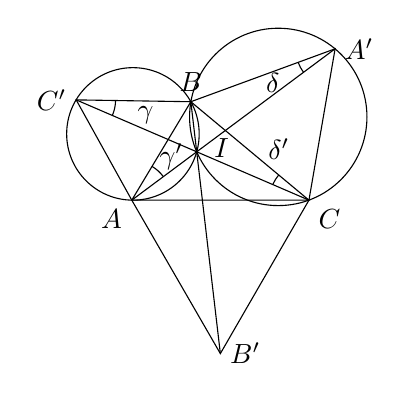
\begin{tikzpicture}[scale=0.5]
			          %projection ($(X)!(B')!(B)$)
			          %nommer chemin 'name path
			          %intersection \path [name intersections={of=d and gb,by=G}];
			          %animation  \draw[visible on=<1>] 
				  %           \draw[visible on=<{2,4}>]
				  %angle arc[radius = 6mm, start angle= 180, end angle= 225] node [below left,pos=0.3]{$\alpha$}
				  %angle \pic [draw, visible on=<2>, above left,"$\beta$", angle eccentricity=1.5] {angle = A'--A--B};
				  %TRIANGLE ABC
				  \coordinate[label=below left:$A$] (A) at (-1.5,0);
				  \coordinate[label=below right:$C$] (C) at (3,0);
				  \coordinate[label=above:$B$] (B) at (0,2.5);
				  \draw (A) -- (B) -- (C) -- cycle;
				  %ABC'
				  \draw (A) let \p1 = ($(B)-(A)$) in -- ++(119:{veclen(\x1,\y1)}) coordinate[label=left:$C'$](C') -- (B);
				  %A'BC
				  \draw (C) let \p1 = ($(B)-(C)$) in -- ++(80.19:{veclen(\x1,\y1)}) coordinate[label=right:$A'$] (A') -- (B);
				  %AB'C
				  \draw (A) let \p1 = ($(A)-(C)$) in -- ++(-60:{veclen(\x1,\y1)}) coordinate[label=right:$B'$] (B') -- (C);
				  %AA', BB', CC'
				  \draw[name path=AA'] (A) -- (A');
				  \draw[name path=BB'] (B) -- (B');
				  \draw (C) -- (C');
				  \path [name intersections={of=AA' and BB',by=I}];
				  \coordinate[label=right:$I$,xshift=1mm,yshift=0.5mm] () at (I);
				  
				  %CERCLE
				  \coordinate (M_1) at ($(A)!0.5!(I)$);
				  \coordinate (M_2) at ($(I)!0.5!(B)$);
				  \path[name path = OM_1] (M_1) -- ($(M_1)!3cm!90:(I)$); 
				  \path[name path = OM_2] (M_2) -- ($(M_2)!3cm!-90:(I)$); 
				  \path [name intersections={of=OM_1 and OM_2,by=O}];
				  \node [draw,visible on=<1>] at (O) [circle through=(A)] {};
				  
				  \coordinate (M_3) at ($(I)!0.5!(C)$);
				  \coordinate (M_4) at ($(C)!0.5!(A')$);
				  \path[name path = O'M_3] (M_3) -- ($(M_3)!3cm!90:(C)$); 
				  \path[name path = O'M_4] (M_4) -- ($(M_4)!3cm!-90:(C)$); 
				  \path [name intersections={of=O'M_3 and O'M_4,by=O'}];
				  \node [draw,visible on=<2>] at (O') [circle through=(A')] {};
				  %ANGLES
				  \pic [draw,"$\gamma$",visible on=<1>, angle eccentricity=1.8] {angle = I--C'--B};
				  \pic [draw,"$\gamma '$",visible on=<1>, angle eccentricity=1.5] {angle = I--A--B};
				  \pic [draw,"$\delta$",visible on=<2>, angle eccentricity=1.8] {angle = B--A'--I};
				  \pic [draw,"$\delta '$",visible on=<2>,above right, angle eccentricity=1.5] {angle = B--C--I};
				  
				  \end{tikzpicture}
				  \end{figure}
				  \vspace{-3mm}
				  \begin{tcolorbox}[basic] 
				      
				    \smallskip
				    \underline{Hypothèses} 
				    \begin{enumerate}
				    \item $\Delta A'BC,\Delta AB'C,\Delta ABC'$ equilatéraux.
				    \end{enumerate}
							      
				    \underline{Thèse}
				    \renewcommand{\theenumi}{\alph{enumi})}
				    \begin{enumerate}
				    \item $|AA'|=|BB'| = |CC'|$,
				    \item $\widehat{BIC}=\widehat{BIA}=120\deg$,
				    \item $AA',BB',CC'$ concourantes.
				    \end{enumerate}

				    \end{tcolorbox}
		
		
		\column{.538\textwidth}\centering
		
		\underline{Résolution}\\ \flushleft
		\onslide<+->Par a), \\ \smallskip 
		$\Delta BCC', \Delta ABA'$ isométriques, \\ \smallskip
		$\rightarrow \gamma = \gamma '$.  \\ \medskip
		Il existe un cercle dont $[BI]$ est une corde et $\gamma,\gamma '$ angles inscrits. \\
		$\rightarrow$ $A,C',B,I$ cocycliques. \\ \medskip
		
		\heart Un quadrilatère convexe inscrit dans un cercle a ses côtés opposés supplémentaires. \\ \medskip
		$\rightarrow$ $\widehat{BIA}=120\deg$. \\ \bigskip
		
		\onslide<+-> De la même façon,
		$\delta = \delta '$. ($\Delta BCC', \Delta ABA'$ isométriques) \\ \medskip
		$\rightarrow$ $A',B,I,C$ cocycliques. \\ \medskip
		$\rightarrow$ $\widehat{BIC}=120\deg$. \hfill $\qed(b)$
		
		
	   \end{columns}   
	   \notedir{%
	   .1 Prouver thèse.
	   .2 $\widehat{BIC}=\widehat{BIA}=120\deg$.
	   .3 Élément de théorie.
	   .4 Côtés opposés d'un quadrilatère convexe inscriptible dans cercle sont supplémentaires..
	   .3 Résolution..
	   .4 De a) $\Delta BCC', \Delta ABA'$ isométriques.
	   .5 $\gamma = \gamma '$..
	   .6 Il existe cercle où $[BI]$ est corde et passant\\ \hspace{5mm} par $C,A'$ d'où on voit $[BI]$ du même angle..
	   .7 Quadrilatère $AC'BI$ est inscriptible dans\\ \hspace{5mm} cercle..
	   .8 $\widehat{BIA}$ est supplémentaire d'un angle de $60\deg$ $\rightarrow$ $\widehat{BIA}=120\deg$..
	   .4 De la même façon, quadrilatère $A'CIB$ inscriptible dans cercle et $\widehat{BIC}=120\deg$..
	   }
    }
    
    \frame{ 
	  % résolution ex1
	  \begin{columns}[t]
		\column{.537\textwidth}\centering 
		

			\underline{Dessin}\\
				  \vspace{-2mm}
				  \begin{figure}[h]
				  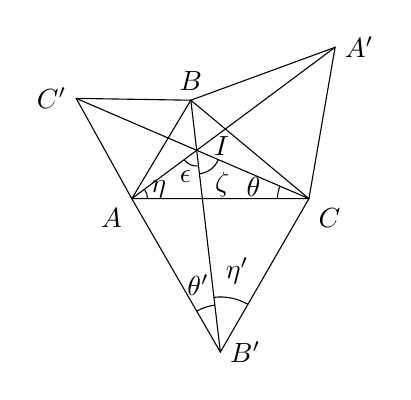
\begin{tikzpicture}[scale=0.5]
			          %projection ($(X)!(B')!(B)$)
			          %nommer chemin 'name path
			          %intersection \path [name intersections={of=d and gb,by=G}];
			          %animation  \draw[visible on=<1>] 
				  %           \draw[visible on=<{2,4}>]
				  %angle arc[radius = 6mm, start angle= 180, end angle= 225] node [below left,pos=0.3]{$\alpha$}
				  %angle \pic [draw, visible on=<2>, above left,"$\beta$", angle eccentricity=1.5] {angle = A'--A--B};
				  %TRIANGLE ABC
				  \coordinate[label=below left:$A$] (A) at (-1.5,0);
				  \coordinate[label=below right:$C$] (C) at (3,0);
				  \coordinate[label=above:$B$] (B) at (0,2.5);
				  \draw (A) -- (B) -- (C) -- cycle;
				  %ABC'
				  \draw (A) let \p1 = ($(B)-(A)$) in -- ++(119:{veclen(\x1,\y1)}) coordinate[label=left:$C'$](C') -- (B);
				  %A'BC
				  \draw (C) let \p1 = ($(B)-(C)$) in -- ++(80.19:{veclen(\x1,\y1)}) coordinate[label=right:$A'$] (A') -- (B);
				  %AB'C
				  \draw (A) let \p1 = ($(A)-(C)$) in -- ++(-60:{veclen(\x1,\y1)}) coordinate[label=right:$B'$] (B') -- (C);
				  %AA', BB', CC'
				  \draw[name path=AA'] (A) -- (A');
				  \draw[name path=BB'] (B) -- (B');
				  \draw (C) -- (C');
				  \path [name intersections={of=AA' and BB',by=I}];
				  \coordinate[label=right:$I$,xshift=1mm,yshift=0.5mm] () at (I);
				  %ANGLES
				  \pic [draw,"$\epsilon$", angle eccentricity=1.8,angle radius=2mm] {angle = A--I--B'};
				  \pic [draw,"$\zeta$", angle eccentricity=1.8,angle radius=3mm] {angle = B'--I--C};
				  \pic [draw,"$\eta$", angle eccentricity=1.8,angle radius=2mm] {angle = C--A--I};
				  \pic [draw,"$\eta'$", angle eccentricity=1.5,angle radius=7mm] {angle = C--B'--I};
				  \pic [draw,"$\theta$", angle eccentricity=1.8,angle radius=4mm] {angle = I--C--A};
				   \pic [draw,"$\theta '$", angle eccentricity=1.5,angle radius=6mm] {angle = I--B'--A};
				  
				  \end{tikzpicture}
				  \end{figure}
				  \vspace{-3mm}
				  \begin{tcolorbox}[basic] 
				      
				    \smallskip
				    \underline{Hypothèses} 
				    \begin{enumerate}
				    \item $\Delta A'BC,\Delta AB'C,\Delta ABC'$ equilatéraux.
				    \end{enumerate}
							      
				    \underline{Thèse}
				    \renewcommand{\theenumi}{\alph{enumi})}
				    \begin{enumerate}
				    \item $|AA'|=|BB'| = |CC'|$,
				    \item $\widehat{BIC}=\widehat{BIA}=120\deg$,
				    \item $AA',BB',CC'$ concourantes.
				    \end{enumerate}

				    \end{tcolorbox}
		
		
		\column{.538\textwidth}\centering
		
		\underline{Résolution}\\ \flushleft
		Par (b), \\ \smallskip
		$\widehat{BIC}=\widehat{BIA}=120\deg \rightarrow \epsilon + \zeta=120\deg$. \\ \medskip
		Par (a), \\ \smallskip 
		$\Delta AA'C, \Delta BB'C$ isométriques, \\ \smallskip
		$\rightarrow \eta = \eta '$.  \\ \medskip
		$\Delta BB'A, \Delta CC'A$ isométriques, \\ \smallskip
		$\rightarrow \theta = \theta '$.  \\ \medskip
		Dans $\Delta IAB'$, \\ \smallskip
		$\epsilon = 180\deg - \eta - 60\deg - \theta'$. \\ \medskip
		Dans $\Delta IB'C$, \\ \smallskip
		$\zeta = 180\deg - \eta ' - 60\deg - \theta$. \\ \bigskip
		
		$\epsilon = \zeta = 60\deg\rightarrow \widehat{BIB'}=180\deg$. \\ \bigskip 
		$AA',BB',CC'$ concourantes. \hfill $\qed(c)$
		
		
		
		
	   \end{columns}   
	   \notedir{%
	   .1 Prouver thèse.
	   .2 $AA',BB',CC'$ concourantes.
	   .3 Élément de théorie.
	   .4 $AA'$, $CC'$ sécantes en $I$.~Montrer que $\widehat{BIB'}=120\deg$ prouve la thèse..
	   .3 Résolution..
	   .4 Déduction de b) que $\epsilon + \zeta=\widehat{AIC}=180\deg$..
	   .4 Déduction de a) que.
	   .5 $\Delta AA'C, \Delta BB'C$ isométriques $\rightarrow \eta = \eta '$..
	   .5 $\Delta BB'A, \Delta CC'A$ isométriques $\rightarrow \theta = \theta '$..
	   .5 Donc $\epsilon = \zeta$ car. 
	   .6 $\epsilon = 180\deg - \eta - 60\deg - \theta'$ dans $\Delta IAB'$..
	   .6 $\zeta = 180\deg - \eta ' - 60\deg - \theta$ dans $\Delta IB'C$..
	   .5 $\rightarrow \epsilon = \zeta = 60\deg$..
	   .4 $\widehat{BIB'}=120 + \epsilon = 180\deg$..
	   .5 $AA',BB',CC'$ concourantes..
	   }
    }
  
\end{document}
